%\documentclass[sigconf, authordraft]{acmart}
\documentclass[sigconf]{acmart}

\usepackage{booktabs} % For formal tables


% Copyright
%\setcopyright{none}
%\setcopyright{acmcopyright}
%\setcopyright{acmlicensed}
\setcopyright{rightsretained}
%\setcopyright{usgov}
%\setcopyright{usgovmixed}
%\setcopyright{cagov}
%\setcopyright{cagovmixed}


% DOI
\acmDOI{}

% ISBN
\acmISBN{978-x-xxxx-xxxx-x/YY/MM}

% Conference
\acmConference[GECCO '19]{the Genetic and Evolutionary Computation Conference 2019}{July 13--17, 2019}{Prague, Czech Republic}
\acmYear{2019}
\copyrightyear{2019}

%\acmArticle{4}
\acmPrice{15.00}

% These commands are optional
%\acmBooktitle{Transactions of the ACM Woodstock conference}
%\editor{Jennifer B. Sartor}
%\editor{Theo D'Hondt}
%\editor{Wolfgang De Meuter}


\begin{document}
\title{Nearest-better Clustering }
\titlenote{Produces the permission block, and
  copyright information}
\subtitle{Subtitle}
\subtitlenote{The full version of the author's guide is available as
  \texttt{acmart.pdf} document}

%%% The submitted version for review should be ANONYMOUS
\author{Ben Trovato}
\authornote{Dr.~Trovato insisted his name be first.}
\orcid{1234-5678-9012}
\affiliation{%
  \institution{Institute for Clarity in Documentation}
  \streetaddress{P.O. Box 1212}
  \city{Dublin} 
  \state{Ohio} 
  \postcode{43017-6221}
}
\email{trovato@corporation.com}

\author{G.K.M. Tobin}
\authornote{The secretary disavows any knowledge of this author's actions.}
\affiliation{%
  \institution{Institute for Clarity in Documentation}
  \streetaddress{P.O. Box 1212}
  \city{Dublin} 
  \state{Ohio} 
  \postcode{43017-6221}
}
\email{webmaster@marysville-ohio.com}

\author{Lars Th{\o}rv{\"a}ld}
\authornote{This author is the
  one who did all the really hard work.}
\affiliation{%
  \institution{The Th{\o}rv{\"a}ld Group}
  \streetaddress{1 Th{\o}rv{\"a}ld Circle}
  \city{Hekla} 
  \country{Iceland}}
\email{larst@affiliation.org}

\author{Valerie B\'eranger}
\affiliation{%
  \institution{Inria Paris-Rocquencourt}
  \city{Rocquencourt}
  \country{France}
}
\author{Aparna Patel} 
\affiliation{%
 \institution{Rajiv Gandhi University}
 \streetaddress{Rono-Hills}
 \city{Doimukh} 
 \state{Arunachal Pradesh}
 \country{India}}
\author{Huifen Chan}
\affiliation{%
  \institution{Tsinghua University}
  \streetaddress{30 Shuangqing Rd}
  \city{Haidian Qu} 
  \state{Beijing Shi}
  \country{China}
}

\author{Charles Palmer}
\affiliation{%
  \institution{Palmer Research Laboratories}
  \streetaddress{8600 Datapoint Drive}
  \city{San Antonio}
  \state{Texas} 
  \postcode{78229}}
\email{cpalmer@prl.com}

\author{John Smith}
\affiliation{\institution{The Th{\o}rv{\"a}ld Group}}
\email{jsmith@affiliation.org}

\author{Julius P.~Kumquat}
\affiliation{\institution{The Kumquat Consortium}}
\email{jpkumquat@consortium.net}

% The default list of authors is too long for headers.
\renewcommand{\shortauthors}{B. Trovato et al.}


\begin{abstract}
This paper provides a sample of a \LaTeX\ document which conforms,
somewhat loosely, to the formatting guidelines for
ACM SIG Proceedings.\footnote{This is an abstract footnote}
\end{abstract}

%
% The code below should be generated by the tool at
% http://dl.acm.org/ccs.cfm
% Please copy and paste the code instead of the example below. 
%
\begin{CCSXML}
<ccs2012>
 <concept>
  <concept_id>10010520.10010553.10010562</concept_id>
  <concept_desc>Computer systems organization~Embedded systems</concept_desc>
  <concept_significance>500</concept_significance>
 </concept>
 <concept>
  <concept_id>10010520.10010575.10010755</concept_id>
  <concept_desc>Computer systems organization~Redundancy</concept_desc>
  <concept_significance>300</concept_significance>
 </concept>
 <concept>
  <concept_id>10010520.10010553.10010554</concept_id>
  <concept_desc>Computer systems organization~Robotics</concept_desc>
  <concept_significance>100</concept_significance>
 </concept>
 <concept>
  <concept_id>10003033.10003083.10003095</concept_id>
  <concept_desc>Networks~Network reliability</concept_desc>
  <concept_significance>100</concept_significance>
 </concept>
</ccs2012>  
\end{CCSXML}

\ccsdesc[500]{Computer systems organization~Embedded systems}
\ccsdesc[300]{Computer systems organization~Redundancy}
\ccsdesc{Computer systems organization~Robotics}
\ccsdesc[100]{Networks~Network reliability}


\keywords{ACM proceedings, \LaTeX, text tagging}


\maketitle

\section{Introduction}

There are many studies on evolutionary algorithms (EAs) solving the real-world optimization problems which are mostly multimodal and complex optimization problems. These problems have not only single global optimum but also many local optima, hence EAs are required to find multiple optima which might be changed as the environment changes. 

To tackle multimodal optimization problems, various niching methods have been proposed. Thomsen proposed the DE extends with a crowding scheme (CDE) \cite{CDE} to replace the high-quality solutions by the most similar candidate solutions. Li proposed the DE with Speciation (SDE) \cite{SDE} to keep a solution away from the nearest neighbor solution when the distance of both solutions is less than a threshold. However, these niching methods are not still enough to find multiple local optima because both of them do not consider searching globally though they consider the solution movement according to the Euclidean distance between the nearest neighbor solutions. For solving this problem, this paper focuses on the Bat Algorithm (BA) \cite{BA} that has the characteristic of echolocation which can predict the distance between bats and the target (\textit{i.e., object/food source}). This algorithm enables bats to estimate the distance between their location and the target even in situations such as the target being surrounded by obstacles and the absence of light. Bats can adjust their velocity which is controlled by their loudness, pulse emission rate and frequency, toward the target. While the iteration search step continues until bats reach the target in the evolutionary process, bats will stop searching the target within its perceptible distance. This research employs a BA which copes with exploitation and exploration search, and extends it with niche radius for multimodal optimization. The niche radius is a threshold distance calculated by the fitness landscape and the number of its peaks.

This paper is organized as follows. After this section, the mechanism of the BA and the proposed algorithm DNRBA are explained in Sections 2 and 3. Section 4 describes the multimodal functions as the test-bed problem in the experiment. Section 5 shows the results while Section 6 discusses them. Finally, this paper concludes in Section 7.

\section{Bat Algorithm}
As mentioned in Section 1, the BA is a metaheuristic algorithm based on the bat behavior with echolocation which are the loudness and the pulse emission rate of the reflect wave controlling the balance between the exploitation and the exploration search. As a bat approaches a better solution than its current solution, the BA turns the loudness $A_i$ up and the pulse rate $r_i$ down. The bats behavior is updated by the following three solution search phases: (i) the bat $i$ flies to the target (\textit{i.e.}, the bat which finds the best solution) with the flight speed controlled by frequency $f_i$; (ii) the bat $i$ flies around the target as a local search; and (iii) the bat $i$ flies randomly in the search space as a global search.

First, in the exploitation phase (i), all bats change their locations $x_i$ with their velocities $v_i$ toward the global best solution. For this calculation, the frequency $f_i$, velocity $v_i$, and location $x_i$, of the bat $i$ are calculated as follows:
\begin{equation}
f_{i} =f_{min}+(f_{max}-f_{min}) \beta
\label{eq:freq} 
\end{equation}

\begin{equation}
v_i^{t+1}=v_i^t+(x_*-x_i^t)* f_i
\label{eq:vi}
\end{equation}
\begin{equation}
x_i^{t+1}=x_i^t+v_i^{t+1}
\label{eq:xi}
\end{equation}
In detail, the new solution $x_i$ is updated by adding the new the velocity ${v_i}$ which is derived from the previous velocity $v_i^t$, the distance between the global best location and the previous location $x_*-x_i^t$, and frequency $f_i$ which range is [${f_{min}}$, ${f_{max}}$] where ${f_{min}}=0$ and ${f_{max}}=1$. $\beta $ is uniform random value from 0 to 1. Next, in the local search phase (ii), the new solution $x_{loc}$ is generated around the global best solution as follows:
\begin{equation}
x_{loc}=x_{*}+ \epsilon A^t \ ,
\label{eq:loc}
\end{equation}
where ${\epsilon}$ is uniform random value within ${[-1,  \ 1]}$. In Eq.(\ref{eq:A}), ${A^t}$ is the averaged loudness of all bats. Finally, in the global search phase (iii), $x_{rnd}$ is generated randomly in the search space as follows:
\begin{equation}
\label{eq:xrnd}
x_{rnd}=x_{lb}+(x_{ub}-x_{lb})*rand(1,D)
\end{equation}
where $x_{ub}$ and $x_{lb}$ describe the upper and lower bounds of the search space, and $rand(1,D)$ is a $D$ dimensional uniform random value within $[0, \ 1]$. 

When a bat finds a better solution than the current one, the loudness $A_i$ and pulse emission rate $r_i$ are updated as follows:
\begin{equation}
A_i^{t+1}=\alpha A_i^t
\label{eq:A}
\end{equation}
\begin{equation}
r_i^{t+1}=r_i^0[1-exp(-\gamma t)]
\label{eq:r}
\end{equation}
Note that the loudness $A_i^0$ is initialized as $A_i^0=1$ and the pulse rate is initialized as a uniform random value $r^0$ whithin $[0, \ 1]$ or a number close around zero. The parameters $\alpha$ and $\gamma$ are the symbolized damping coefficients. The pseudo code of the BA is given in the Algorithm 1 and its brief summary is described below.

\begin{itemize}
\item STEP1: Population initialization of bats (line 1 to 3)\\
The population of bats ${x_i}(i=1, 2, ..., N)$, the loudness ${A_i^0}$, the pulse rate ${r_i^0}$ are initialized as the initial values. The frequency ${f_i}$ is initialized by Eq.(\ref{eq:freq}).
\item STEP2: New solution updates (line 6)\\
The new solutions ${x_i}$ is calculated by Eqs. (\ref{eq:vi}) and (\ref{eq:xi}).
\item STEP3: New solution generation around the global best solution ${x_*}$ (line 7 to 9)\\
A new solution $x_{loc}$ is generated around $x_*$ by Eq. (\ref{eq:loc}) when the pulse emission rate $r_i$ is lower than a random value.
\item STEP4: Random new solution generation (line 10)\\
A new solution ${x_{rnd}}$ is generated randomly by Eq. (\ref{eq:xrnd}).  
\item STEP5: Solutions update(line 11 to 14)\\
When ${rand < A_i}$, the best solution is selected from $x_i$, ${x_{loc}}$, and ${x_{rnd}}$ by Eqs.(\ref{eq:A}) and (\ref{eq:r})
\item STEP6: Return to STEP2 
\end{itemize}

\begin{algorithm}[H]
\caption{Bat Algorithm}
\label{code:ba}
\begin{algorithmic}[1]
\REQUIRE Objective\ Function\ $F(x)$
\STATE Initialize Population $x_i(i=1,2,..., N)$ and $v_i$\\
\STATE Define frequency $f_i$ at location $x_i$ [eq.(\ref{eq:freq})]
\STATE Initialize pulse rates $r_i$, and loudness $A_i$
\WHILE{($t <$ Max number of iterations)}
\FOR{i=1 to N}
\STATE Generate a new solution $x_i$ and velocity $v_i$ [eqs.(\ref{eq:vi}),(\ref{eq:xi})]
\IF{($rand>r_i$)}
\STATE Generate a new solution $x_{loc}$ around a global best solution $x_i$ [eq.(\ref{eq:loc})] 
% \ELSE
% \STATE Continue
\ENDIF
\STATE Generate a new solution $x_{rnd}$ randomly
\IF{($rand<A_i \& \min (F(x_i), F(x_{loc}), F(x_{rnd})<F(x_{i*})$)}
\STATE Accept the new solution, and update pulse rate $r_i$ \\ \& loudness $A_i$ [eqs. (\ref{eq:A})(\ref{eq:r})]  
\ENDIF
\STATE Evaluate all bats and select a best solution $x_*$ in the current solutions
\ENDFOR
\ENDWHILE
\end{algorithmic}
\end{algorithm}

\section{Sharing Scheme}
The first sharing mechanism was proposed by Holland \cite{SH01} to spread individuals widely in multimodal optimization. The concept of a sharing scheme is to reduce the fitness value of similar individuals and classify these individuals within the population.
\subsection{Niche Radius}
The \textit{niche radius} is the distance calculated by the upper and lower bounds of the search space. The equation is defined by:
\begin{equation}
\label{eq:dist}
dist =\frac{1}{2} \sqrt{(x_{ub}-x_{lb})^2}
\end{equation}
\begin{equation}
\label{eq:nr}
\sigma=\frac{dist}{\sqrt[D]{q}},
\end{equation}
where $x_{ub}, x_{lb}$ are the upper and lower bounds of the $D$ dimension in the search space, and $q$ is the number of peaks of the fitness landscape.

\subsection{Fitness Sharing}
\textit{Fitness Sharing} is derived from the concept of a \textit{crowding scheme} \cite{crowding} replacing a new individual by nearby similar individual in the population. The most widely used \textit{sharing function} is given as follows:
\begin{equation}
\label{eq:sh}
sh(d_{ij})= \begin{cases}
1-(\frac{d_{ij}}{\sigma})^\alpha & ({\rm if} \ d_{ij} < \sigma) \\
0 & ({\rm otherwise})
\end{cases}
\end{equation}
where $d_{ij}$ is the distance between individuals $i,j$, and $\sigma$ is the niche radius defined above in Eq.(\ref{eq:nr}) as the threshold. $\alpha$ is the coefficient parameter, basically set to 1. By the \textit{sharing function}, the \textit{niche count} which represents the density of nearby similar individuals, is defined by:
\begin{equation}
\label{eq:nc}
m_i=\sum_{j=1}^N sh(d_{ij})
\end{equation}
Subsequently, \textit{The shared fitness} $\phi_i$ is given by:
\begin{equation}
\label{sf}
\phi_i=\frac{F_i}{m_i}
\end{equation}
where $F_i$ is the raw fitness value of the individual and $m_i$ is the niche count. \textit{the shared fitness} indicates the fitness of the individual considering the density of similar individuals.

\subsection{Dynamic Niche Sharing}
In order to cut off the redundancy of the \textit{shared fitness}, \textit{dynamic niche sharing} is proposed by Miller in \cite{DNS}. This scheme enables to identify the $q$ peaks of the fitness landscape and classify all individuals into several groups in the same domain with the radius dynamically.
\begin{equation}
\label{eq:dns}
m_i^{dyn} = \begin{cases}
n_j & ({\rm if \ individual \ } i {\rm \ is \ within \ the \ dynamic \ niche \ } $j$) \\
m_i & ({\rm otherwise})
\end{cases}
\end{equation}
where $n_j$ is the $j-th$ niche radius and $m_i$ is the \textit{niche count} defined in Eq.(\ref{eq:nc}) as mentioned above. The \textit{shared fitness} is calculated as follows:
\begin{equation}
\label{dsf}
\phi_i^{dyn}=\frac{F_i}{m_i^{dyn}}
\end{equation}

\section{Proposed Algorithm}
\subsection{Bat Algorithm with Dynamic Niche Radius}
In our algorithm, we provide a new \textit{dynamic niche radius} to classify all individuals into several groups by the density of some of them in the same domain with niche radius to avoid overlapping the same peak in the fitness landscape. The new \textit{dynamic niche radius} is updated each iteration step as follows:
\begin{equation}
\label{eq:dnr}
m_i^{dyn}= \begin{cases}
\sigma & ({\rm if} \ m_{i} < \sigma) \\
m_i & ({\rm otherwise})
\end{cases}
\end{equation}

By this equation, the movement of solutions is given by
\begin{equation}
\label{eq:dnrvi}
v_i^{t+1}=v_i^t+(x_i^t-x_{NR*})*f_i
\end{equation}
\begin{equation}
\label{eq:dnrxi}
x_i^{t+1}= \begin{cases}
x_i^t+v_i^{t+1} & ({\rm if} \ d_{ij}^t < m_i^{dyn}) \\
x_i^t & ({\rm otherwise})
\end{cases}
\end{equation}
where $x_{NR*}$ is the best solution in the domain of the niche radius and $d_{ij}^t$ indicates the Euclidean distance between the nearest neighbor solutions. 

In the local search phase, the new solution $x_{loc}$ is generated around the best solution $x_{NR*}$ in the domain of the radius as follows:
\begin{equation}
\label{eq:dnrloc}
x_{loc}=x_{NR*} + A_i^t*rand(1,D,[-m_i, m_i])
\end{equation}
where $A_i$ are the same values as in the BA.
In the global search phase, the new solution $x_{rnd}$ is generated randomly in all domains of the dynamic niche radius as follows: 
\begin{equation}
\label{eq:dnrrnd}
x_{rnd}=x_i^t + rand(1,D,[-m_i, m_i])
\end{equation}

% Fig. \ref{fig:niche} provides an example to illustrate the solution movement to keep the solution $x_i$ from the best solution $x_{NR*}$ in the domain of the radius, where the red circle and the yellow star indicates solution $x_i$ and the best solution $x_{NR*}$. This figure shows the situation that the solutions $x_1, x_2 $ and $ x_3$ are located in the area of $x_{NR*}$ with the radius. In this case, these solutions are moved out from the area of the best solution $x_{NR*}$.
\subsection{Algorithm Description}
The pseudo codes of the Dynamic Niche Radius and DNRBA are given in Algorithm 2 and 3. Its brief summary is described below.
\begin{algorithm}[t]
\caption{Dynamic Niche Radius}
\label{code:dnr}
\begin{algorithmic}[2]
\REQUIRE Current Population $x_i(i=1,2,..., N)$ and $v_i$
\FOR{i=1 to N}
\FOR{j=1 to N}
\STATE Calculate $d_{ij}$ between individuals $i,j$
\IF{( $d_{ij} < \sigma$)}
\STATE $sh(d_{ij}) =  (1-\frac{d_{ij}}{\sigma})$ [Eq.(\ref{eq:sh})]
\ELSE
\STATE $sh(d_{ij}) =  0 $ [Eq.(\ref{eq:sh})]
\ENDIF
\ENDFOR
\STATE $m_i=\sum_{j=1}^N sh(d_{ij})$ [Eq.(\ref{eq:nc})]
\ENDFOR
\FOR{i=1 to N}
\IF{$(m_i < \sigma)$}
\STATE $m_i^{dyn}=\sigma$ [Eq.(\ref{eq:dnr})]
\ELSE 
\STATE $m_i^{dyn} = m_i$ [Eq.(\ref{eq:dnr})]
\ENDIF
\ENDFOR
\RETURN Dynamic Niche Radius $m_i^{dyn}$

\end{algorithmic}
\end{algorithm}


\begin{algorithm}[t]
\caption{Bat Algorithm with Dynamic Niche Radius (DNRBA)}
\label{code:dnrba}
\begin{algorithmic}[3]
\REQUIRE Objective\ Function\ $F(x)$
\STATE Initialize Population $x_i(i=1,2,..., N)$ and $v_i$\\
\STATE Define frequency $f_i$ at location $x_i$ [Eq.(\ref{eq:freq})]
\STATE Initialize pulse rates $r_i$, and loudness $A_i$
\WHILE{($t <$ Max number of iterations)}
\STATE Calculate Dynamic Niche Radius (Algorithm 2)
\FOR{i=1 to N}
\STATE Generate a new solution $x_i$ and velocity $v_i$ [Eqs.(\ref{eq:dnrvi}) and (\ref{eq:dnrxi})]
\IF{($rand>r_i$)}
\STATE Generate a new solution $x_{loc}$ around a global best solution $x_i$ [Eq.(\ref{eq:dnrloc})] 
% \ELSE
% \STATE Continue
\ENDIF
\STATE Generate a new solution $x_{rnd}$ randomly [Eq.(\ref{eq:dnrrnd})]
\IF{($rand<A_i \& \min (F(x_i), F(x_{loc}), F(x_{rnd})<F(x_{i*})$)}
\STATE Accept the new solution, and update pulse rate $r_i$ \\ \& loudness $A_i$ [Eqs. (\ref{eq:A}) and (\ref{eq:r})]  
\ENDIF
\STATE Evaluate all bats and select a best solution $x_*$ in the current solutions
\ENDFOR
\ENDWHILE
\end{algorithmic}
\end{algorithm}

\begin{itemize}
\item STEP1: Population initialization of bats (line 1 to 3)\\
The population of bats ${x_i}(i=1, 2, ..., N)$, the loudness ${A_i^0}$, the pulse rate ${r_i^0}$ are initialized as the initial values. The frequency ${f_i}$ is initialized by Eq.(\ref{eq:freq}).
\item STEP2: Calculate dynamic niche radius $m_i^{dyn} $(line 5) 
\item STEP3: New solution updates (line 7)\\
The new solutions ${x_i}$ are calculated by Eqs. (\ref{eq:vi}) and (\ref{eq:xi}).
\item STEP4: New solution generation around the best solution ${x_{NR*}}$ (line 8 to 11)\\
A new solution $x_{loc}$ is generated around $x_*$ by Eq. (\ref{eq:loc}) when the pulse emission rate $r_i$ is lower than a random value.
\item STEP5: Random new solution generation (line 11)\\
A new solution ${x_{rnd}}$ is generated randomly by Eq. (\ref{eq:xrnd}).  
\item STEP6: Solutions update (line 15 to 16)\\
When ${rand < A_i}$, the best solution is selected from $x_i$, ${x_{loc}}$, and ${x_{rnd}}$ by Eqs.(\ref{eq:A}) and (\ref{eq:r})
\item STEP7: Return to STEP2 
\end{itemize}


\section{Experimental Procedure}
To measure the number of local optima and the convergence speed, we compare the performance of the BA with the DNRBA. In this section, two multimodal functions which Griewank function has both global and local optima and Shubert function has only global optima, are employed for minimization \cite{f1}\cite{TSC2}.

\subsection{Multimodal Test Functions}
\begin{description}
\item[$F_1$: Griewank Function]\mbox{}\\
This function is described as follows as shown in Fig. \ref{fig:f1}.
\begin{equation}
F_1(x)= \sum_{i=1}^D \frac{x_{i}}{4000} - \prod_{i=1}^D \cos(\frac{x_i}{\sqrt{i}}) + 1,
\label{eq:f1}
\end{equation}
The fitness value of the global optima is ${F(x_*)}=0$. This function has 17 optima (1 global optimum and 16 local optima) in the range between $x_1, x_2 \in [-10, \ 10]$.

\begin{figure}[h]
\centering
\subfigure[Fitness landscape]{
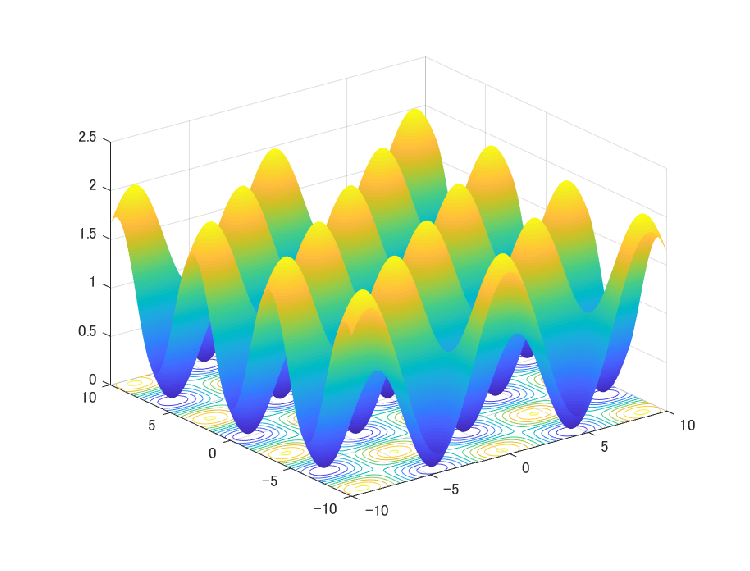
\includegraphics[width=0.8\linewidth]{eps/3d_griewank.eps}
\label{fig:3df1}}
\subfigure[Contour plot]{
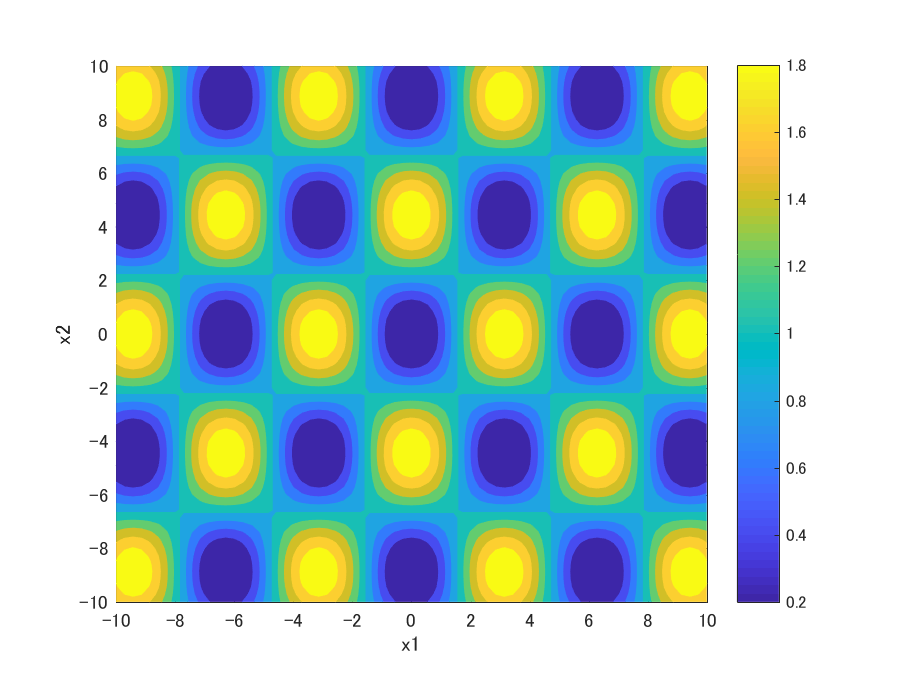
\includegraphics[width=0.8\linewidth]{eps/cont_griewank.eps}
\label{fig:cf1}}

\caption{$F_1$: Griewank Function}
\label{fig:f1}
\end{figure}

\item[$F_2$: Shubert Function]\mbox{}\\
 This function is described as follows as shown in Fig. \ref{fig:f2}.
 \begin{equation}
F_2(x) = \prod_{i=1}^D \sum_{j=1}^5 j \cos[(j+1)x_i+j], 
\end{equation}
where $D$ is the number of dimensions and the fitness value of the global optima is ${F(x_*)=-187.731}$. This function has  $D \cdot 3^D $ global optima in the range of the search space $x_i \in [-10, 10]^D$ with $i=1,2,...,D$. Fig. \ref{fig:f2} shows an example of the Shubert 2D function which has 18 global optima. 

\begin{figure}[h]
\centering
\subfigure[Fitness landscape]{
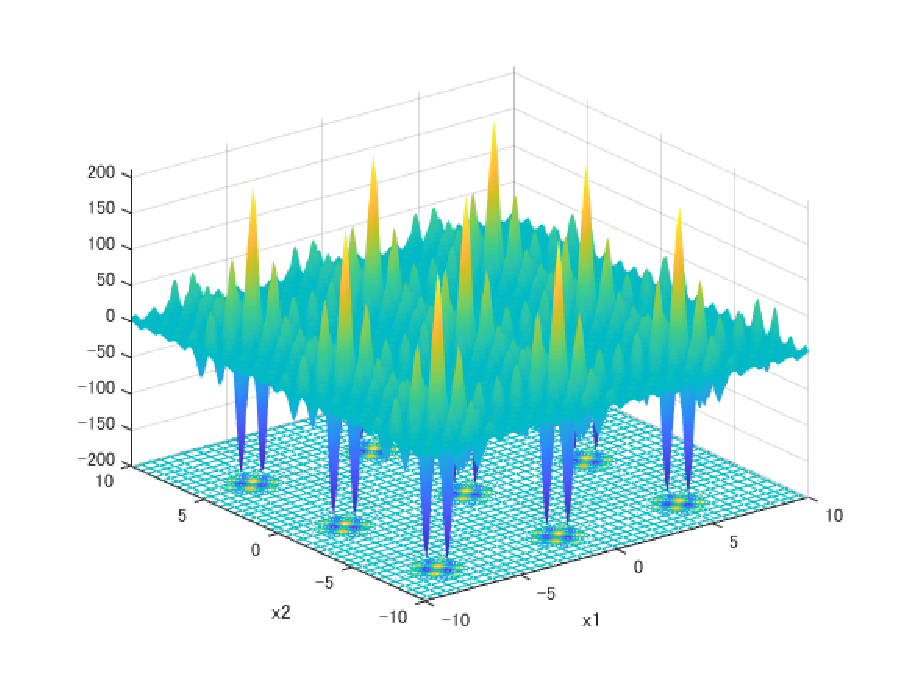
\includegraphics[width=0.8\linewidth]{eps/3d_shubert.eps}
\label{fig:3df2}}
\subfigure[Contour plot]{
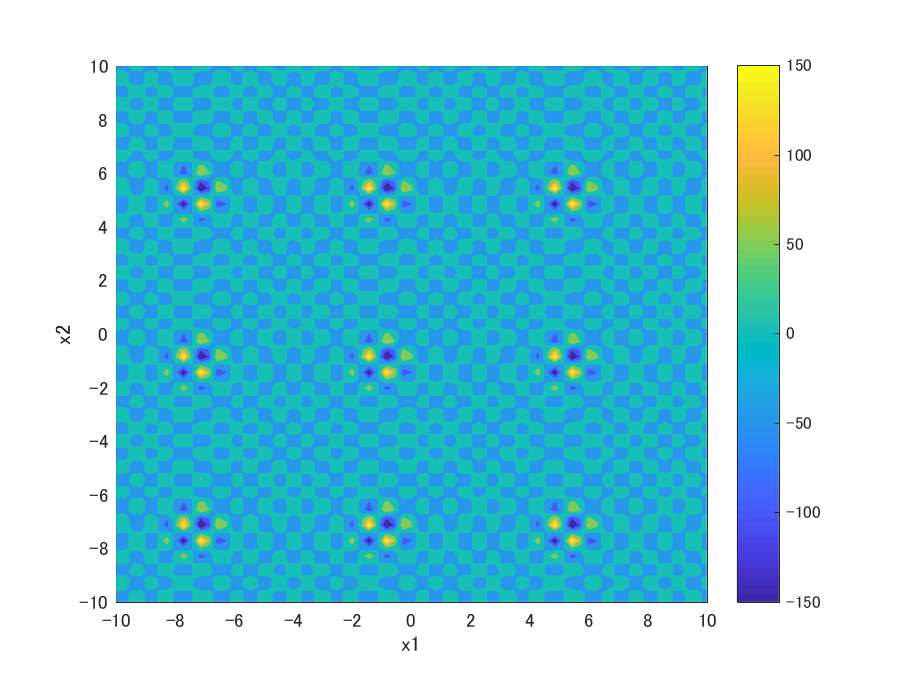
\includegraphics[width=0.8\linewidth]{eps/cont_shubert.eps}
\label{fig:cf2}}

\caption{$F_2$: Shubert Function}
\label{fig:f2}
\end{figure}

\end{description}
% \begin{figure}[h]
% \begin{center}
% \begin{tabular}{c}
% \begin{minipage}{0.5\hsize}
% \begin{center}
% 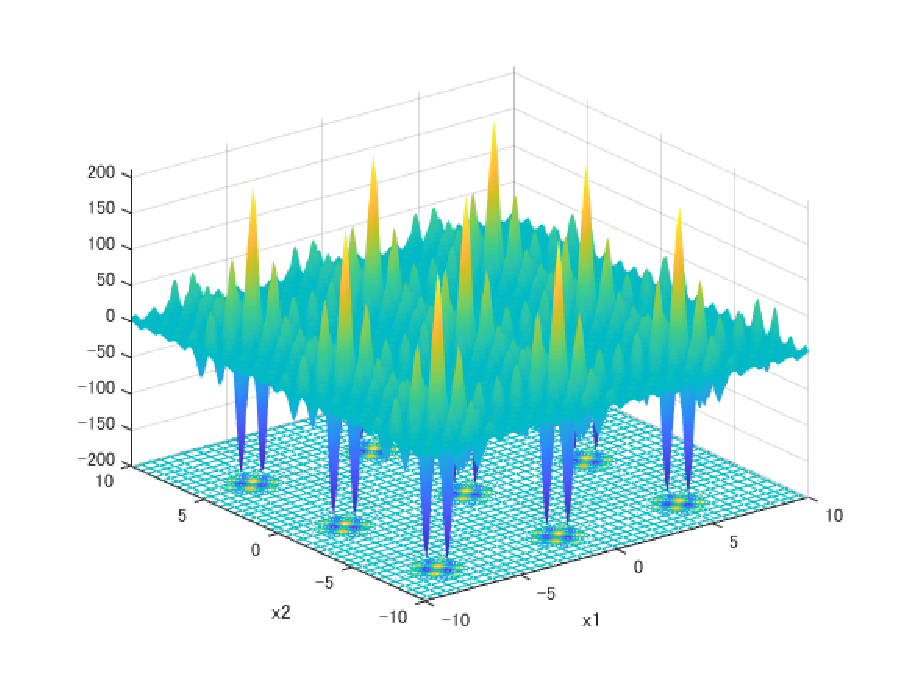
\includegraphics[width=1.0\linewidth]{eps/3d_shubert.eps}
% \hspace{1.6cm} (a) The fitness landscape
% \label{fig:3d_shubert}
% \end{center}
% \end{minipage}
% \begin{minipage}{0.5\hsize}
% \begin{center}
% 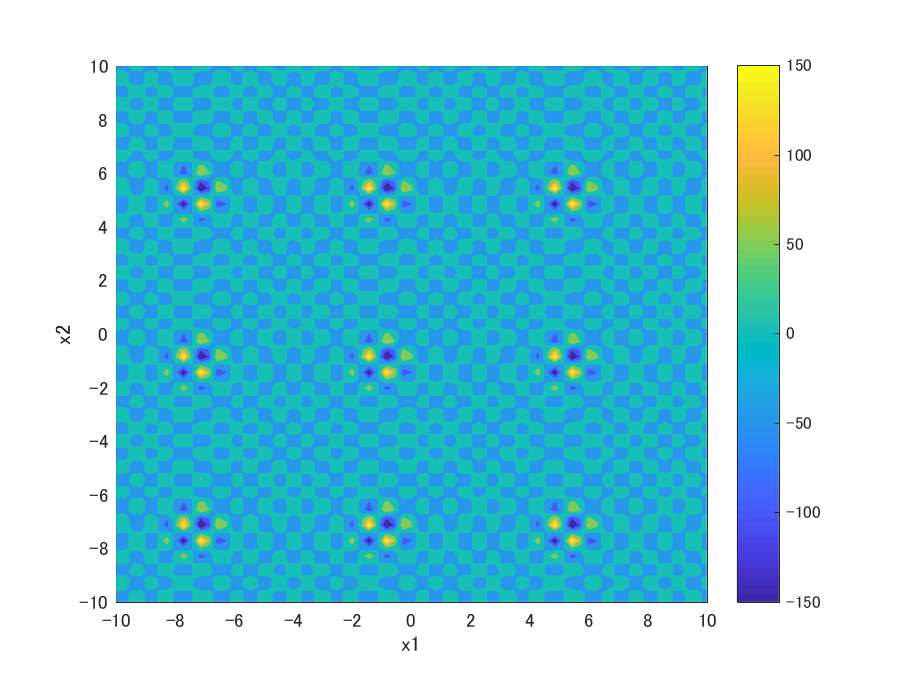
\includegraphics[width=1.0\linewidth]{eps/cont_shubert.eps}
% \hspace{1.6cm} (b) The contour plot
% \label{fig:cont_shubert}
% \end{center}
% \end{minipage}
% \end{tabular}
% \caption{Shubert}
% \label{fig:f2}
% \end{center}
% \end{figure}

\subsection{Experimental Measurement}
\subsubsection{Peak Ratio}
This experiment employs Peak Ratio (PR) \cite{CDE} as the evaluation criterion in the CEC (\textit{IEEE Congress on Evolutionary Computation}) 2013 competition \cite{cec2013}. The PR value measures the ratio of the found global and local optima in the total number of true peaks and it is calculated as follows: 
\begin{equation}
\label{eq:PR}
PR=\frac{\sum_{run=1}^{MR}FPs}{TP*MR}
\end{equation}
 where ${MR}$ indicates the maximum run, ${FPs}$ indicates the number of peaks found by the optimization algorithm. ${TP}$ indicates the number of all known peaks of the function. We define that the peak is found when the Euclidean distance between the all known peaks and the nearest solution calculated by the optimization algorithm is less than the thresholds $\varepsilon = \{1.0E-1, 1.0E-2\}$.

\subsubsection{Peak Accuracy}
To measure how close solutions are close to the peaks (global and local optima), we employ Peak Accuracy (PA) \cite{CDE} calculated as follows:
\begin{equation}
PA=\sum_{j=1}^{TP}|F(s_j)-F(x_{NN_j})|,
\end{equation}
where $s_j$ and $x_{NN_j}$ denote the each known peak and the nearest neighbor solution. As the closest distance between both of them is short, the value of PA is close to 0. 

 \subsection{Experimental Parameters}
We employ the parameters as follows: frequency $f_{max}=1$, $f_{min}=0$, loudness ${A^0}=1$, parse rate ${r^0} \in [0, \ 1]$ with ${\alpha =\gamma = 0.9}$. The population size ${N=100}$. This experiments are conducted with 30 runs with different random seeds and 30000 evaluations as the termination condition for each run.

\section{Results and Analysis}
To test the effect of the DNRBA mechanism, this section investigates the peak ratio (PR) and the peak accuracy (PA) of each benchmark test function. Table \ref{tab1} and \ref{tab2} show the results that the PR and the PA values of two algorithms based on the settings of averaged over 30 individual runs at the final iteration. Fig. \ref{fig:results_ba} and \ref{fig:results_dnrba} show that the solutions are distributed at the final iteration for all functions.

\subsection{Peak Ratio}
The case of $\varepsilon=1.0E-1$ from Table \ref{tab1}, the PR values of DNRBA were greatly higher than BA in $F_1$. It can be seen that DNRBA found almost all global and local optima, as shown in Fig. \ref{fig:f1dnrba}. Although Fig. \ref{fig:f2dnrba} appears to locate solutions at all peaks, the values of DNRBA were less than BA in $F_2$, because $F_2$ has an extremely sharp and complex landscape. Moreover, the exploitation of BA outperformed that of DNRBA so that $F_2$ is for finding only global optima (\textit{not searching local optima}). Table \ref{tab2} shows the results of the case of $\varepsilon=1.0E-2$. The value of DNRBA is the same as $\varepsilon=1.0E-1$ in $F_1$. However, DNRBA remarkably decreased from 0.4241 to 0.0426 in $F_2$. It can be seen that the exploitation of DNRBA is not efficient to reach the peaks precisely.  

\subsection{Peak Accuracy}
DNRBA outperformed BA for $F_1$ from Table \ref{tab1} and \ref{tab2} in $\varepsilon=1.0E-1, 1.0E-2$ to find global and local optima. In contrast, the PA value of BA was better than DNRBA in $F_2$. BA enables to locate all solutions at all peaks from Fig. \ref{fig:f2ba}. As well as Fig. \ref{fig:f2dnrba}, although DNRBA seems to locate at several global optima (several solutions are located at no peaks), the value of DNRBA is lower than BA.
\begin{table*}[h]
\caption{Peak Ratio and Peak Accuracy of BA and DNRBA (averaged over 30 runs)}
\begin{center}
\begin{tabular}{c|c|c|c|c}
\multicolumn{5}{c}{$\varepsilon = 1.0E-1$} \\
\hline
\multicolumn{1}{c|}{} & \multicolumn{2}{c|}{BA} & \multicolumn{2}{c}{DNRBA} \\
\hline
 & PR & PA & PR & PA \\

Function & (Mean and SD) & (Mean and SD) & (Mean and SD) & (Mean and SD) \\
\hline
$F_1 $ & 0.2725 $\pm$ 0.0598 & 0.2416 $\pm$ 0.0149 & {\bf 0.9373} $\pm$ 0.1176  & {\bf 0.0094} $\pm$ 0.0155  \\
\hline
$F_2 $ & {\bf 0.4889} $\pm$ 0.1819 & {\bf 1.8160} $\pm$ 0.4990 & 0.4241 $\pm$ 0.388 & 2.4123 $\pm$ 0.6780 \\
\hline

\end{tabular}
\label{tab1}
\end{center}
\end{table*}

\begin{table*}[h]
\caption{Peak Ratio and Peak Accuracy of BA and DNRBA (averaged over 30 runs)}
\begin{center}
\begin{tabular}{c|c|c|c|c}
\multicolumn{5}{c}{$\varepsilon = 1.0E-2$} \\
\hline
\multicolumn{1}{c|}{} & \multicolumn{2}{c|}{BA} & \multicolumn{2}{c}{DNRBA} \\
\hline
 & PR & PA & PR & PA \\

Function & (Mean and SD) & (Mean and SD) & (Mean and SD) & (Mean and SD) \\
\hline
$F_1 $ & 0.2725 $\pm$ 0.0608 & 0.2416 $\pm$ 0.0151 & {\bf 0.9373} $\pm$ 0.1176  & {\bf 0.0094} $\pm$ 0.0155  \\
\hline
$F_2 $ & {\bf 0.0556} $\pm$ 0.0619 & {\bf 1.8160} $\pm$ 0.4990 & 0.0426 $\pm$ 0.0477 & 2.4123 $\pm$ 0.6780 \\
\hline

\end{tabular}
\label{tab2}
\end{center}
\end{table*}

\begin{figure}[h]
\centering
\subfigure[$F_1$]{
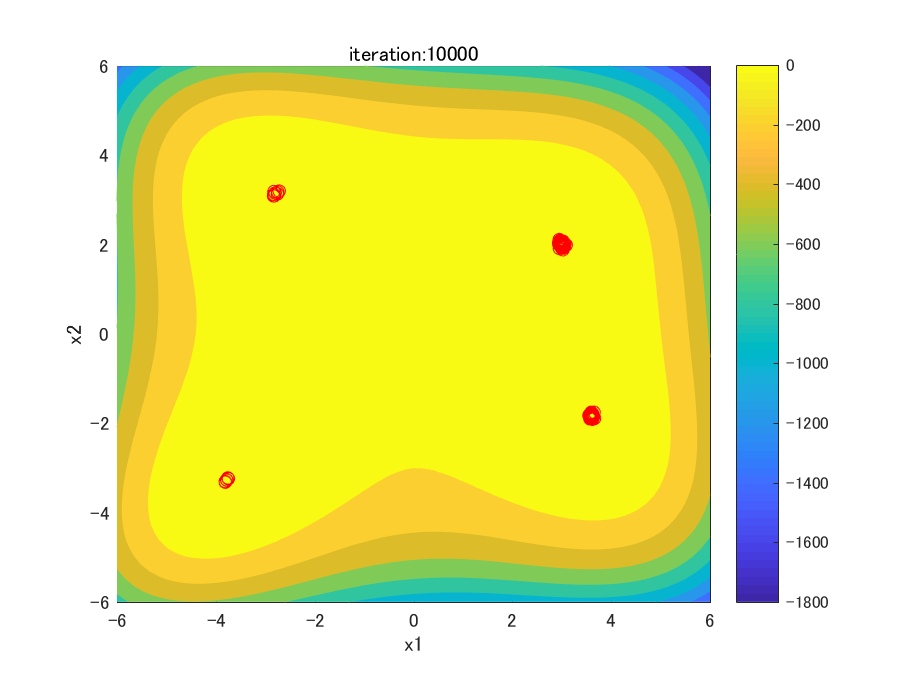
\includegraphics[width=0.8\linewidth]{eps/f1_ba.eps}
\label{fig:f1ba}}
\subfigure[$F_2$]{
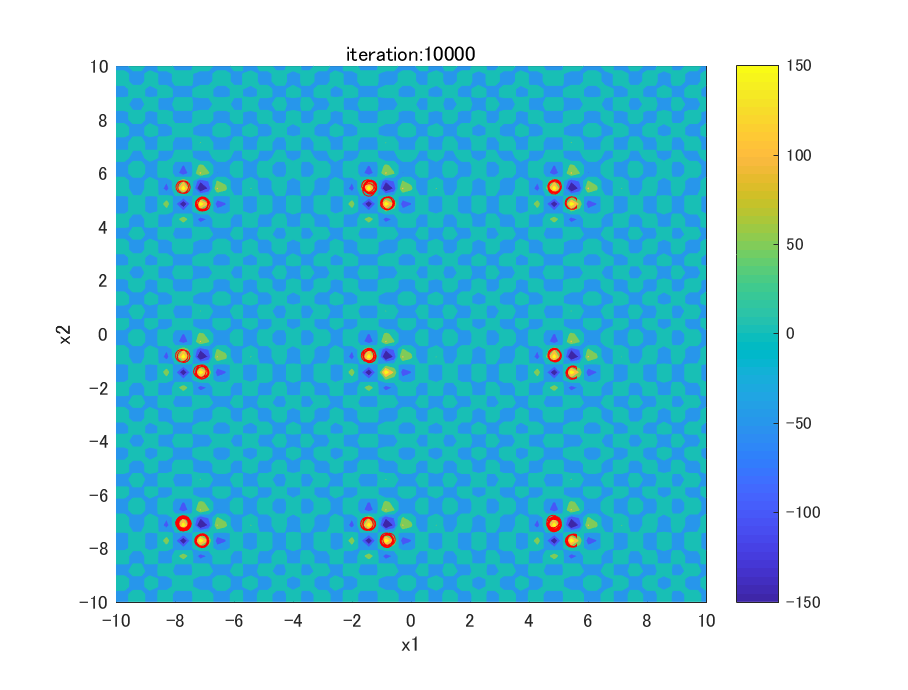
\includegraphics[width=0.8\linewidth]{eps/f2_ba.eps}
\label{fig:f2ba}}

\caption{BA}
\label{fig:results_ba}
\end{figure}

\begin{figure}[h]
\centering
\subfigure[$F_1$]{
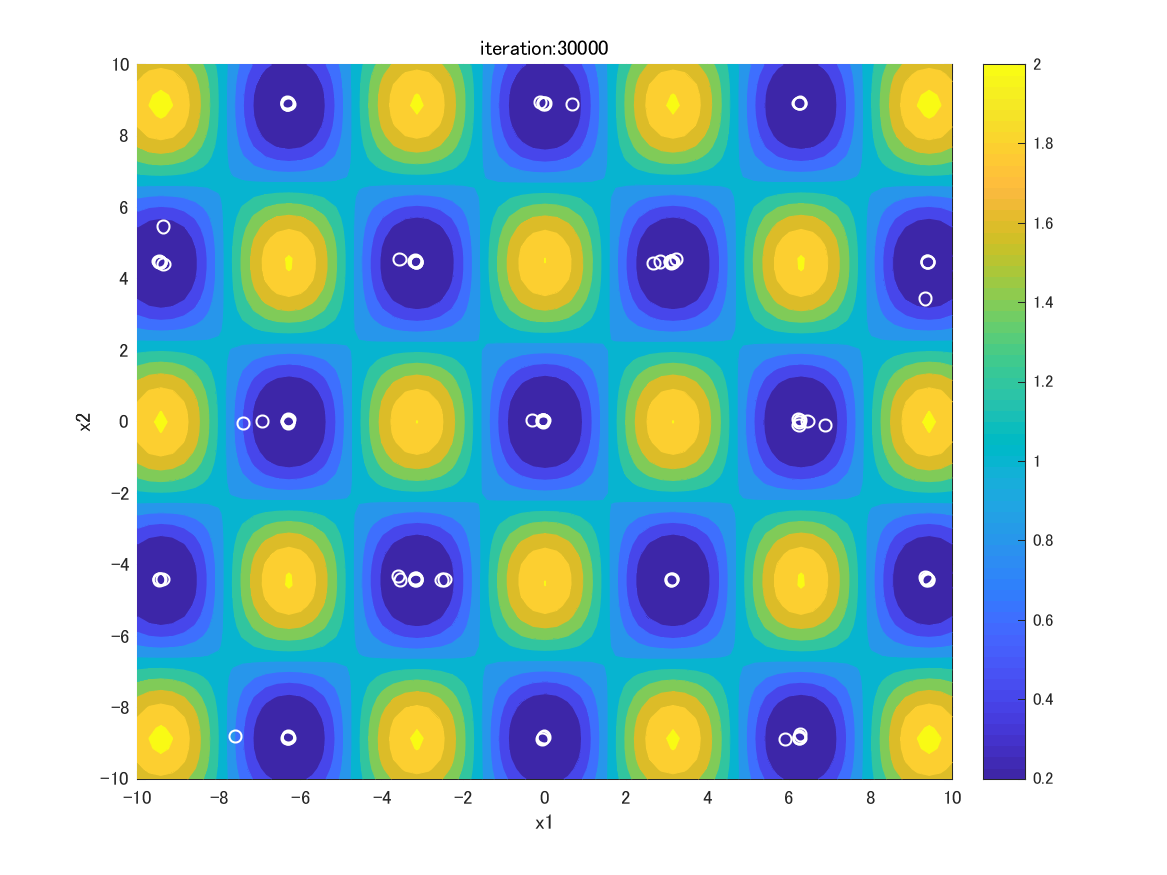
\includegraphics[width=0.8\linewidth]{eps/f1_dnrba.eps}
\label{fig:f1dnrba}}
\subfigure[$F_2$]{
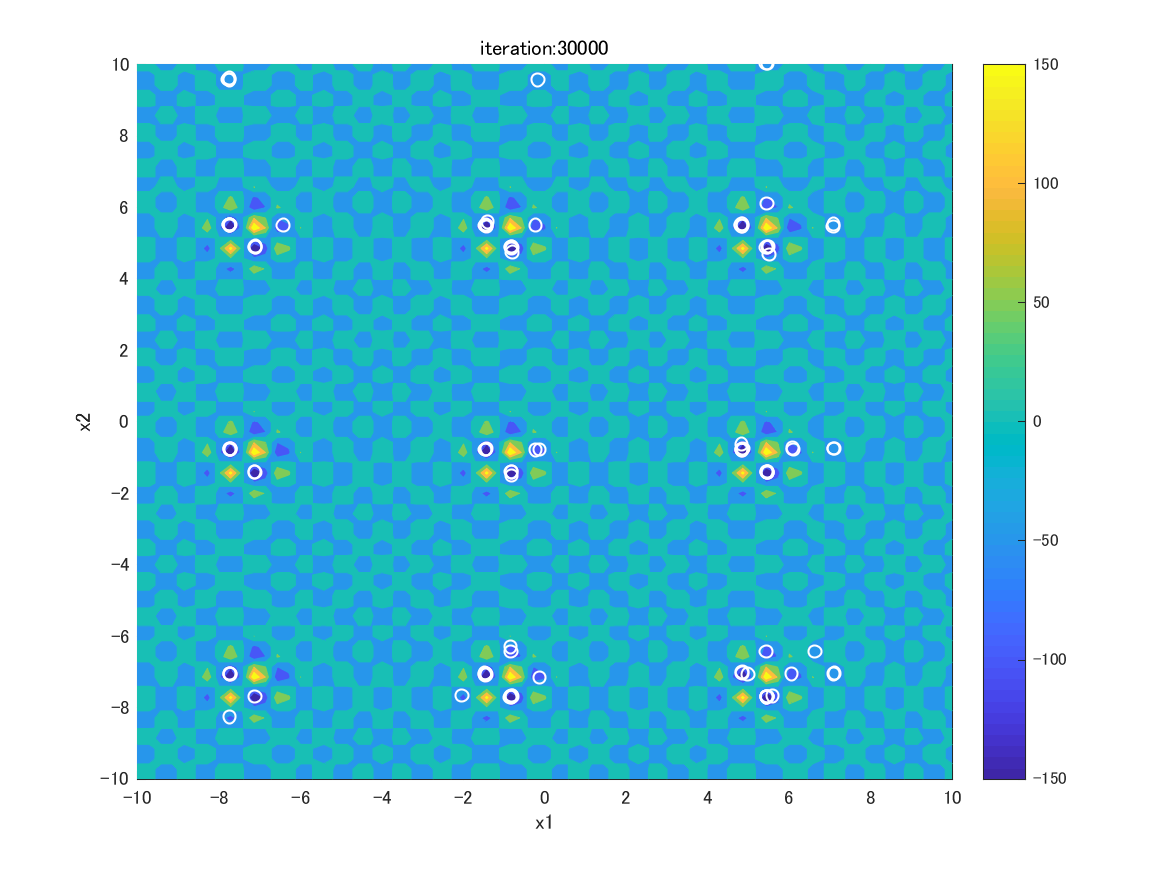
\includegraphics[width=0.8\linewidth]{eps/f2_dnrba.eps}
\label{fig:f2dnrba}}

\caption{DNRBA}
\label{fig:results_dnrba}
\end{figure}

\section{Conclusion}
This paper proposed BA extended with a Dynamic Niche Radius which enables the solutions to avoid overlapping  into the same peak, and to locate multiple global optima in several multimodal functions. To evaluate the performance of DNRBA, this algorithm were compared with BA. The results show that NRBA outperformed at not only global optima but also local optima in the fitness landscape, because the spatial distribution mechanism in DNRBA copes with the trade-off between the exploration and the exploitation. In contrast, BA is still better than NRBA regarding the exploitation due to converge to a single global best solution. In future work, we will compare DNRBA with current state-of-the-art algorithms and apply it for dynamic optimization problems.

% \subsection{Citations}
% Citations to articles~\cite{bowman:reasoning,
% clark:pct, braams:babel, herlihy:methodology},
% conference proceedings~\cite{clark:pct} or maybe
% books \cite{Lamport:LaTeX, salas:calculus} listed
% in the Bibliography section of your
% article will occur throughout the text of your article.
% You should use BibTeX to automatically produce this bibliography;
% you simply need to insert one of several citation commands with
% a key of the item cited in the proper location in
% the \texttt{.tex} file~\cite{Lamport:LaTeX}.
% The key is a short reference you invent to uniquely
% identify each work; in this sample document, the key is
% the first author's surname and a
% word from the title.  This identifying key is included
% with each item in the \texttt{.bib} file for your article.

% The details of the construction of the \texttt{.bib} file
% are beyond the scope of this sample document, but more
% information can be found in the \textit{Author's Guide},
% and exhaustive details in the \textit{\LaTeX\ User's
% Guide} by Lamport~\shortcite{Lamport:LaTeX}.

% This article shows only the plainest form
% of the citation command, using \texttt{{\char'134}cite}.

% Some examples.  A paginated journal article \cite{Abril07}, an enumerated
% journal article \cite{Cohen07}, a reference to an entire issue \cite{JCohen96},
% a monograph (whole book) \cite{Kosiur01}, a monograph/whole book in a series (see 2a in spec. document)
% \cite{Harel79}, a divisible-book such as an anthology or compilation \cite{Editor00}
% followed by the same example, however we only output the series if the volume number is given
% \cite{Editor00a} (so Editor00a's series should NOT be present since it has no vol. no.),
% a chapter in a divisible book \cite{Spector90}, a chapter in a divisible book
% in a series \cite{Douglass98}, a multi-volume work as book \cite{Knuth97},
% an article in a proceedings (of a conference, symposium, workshop for example)
% (paginated proceedings article) \cite{Andler79}, a proceedings article
% with all possible elements \cite{Smith10}, an example of an enumerated
% proceedings article \cite{VanGundy07},
% an informally published work \cite{Harel78}, a doctoral dissertation \cite{Clarkson85},
% a master's thesis: \cite{anisi03}, an online document / world wide web
% resource \cite{Thornburg01, Ablamowicz07, Poker06}, a video game (Case 1) \cite{Obama08} and (Case 2) \cite{Novak03}
% and \cite{Lee05} and (Case 3) a patent \cite{JoeScientist001},
% work accepted for publication \cite{rous08}, 'YYYYb'-test for prolific author
% \cite{SaeediMEJ10} and \cite{SaeediJETC10}. Other cites might contain
% 'duplicate' DOI and URLs (some SIAM articles) \cite{Kirschmer:2010:AEI:1958016.1958018}.
% Boris / Barbara Beeton: multi-volume works as books
% \cite{MR781536} and \cite{MR781537}.

% A couple of citations with DOIs: \cite{2004:ITE:1009386.1010128,
%   Kirschmer:2010:AEI:1958016.1958018}.

% Online citations: \cite{TUGInstmem, Thornburg01, CTANacmart}.


% \subsection{Tables}
% Because tables cannot be split across pages, the best
% placement for them is typically the top of the page
% nearest their initial cite.  To
% ensure this proper ``floating'' placement of tables, use the
% environment \textbf{table} to enclose the table's contents and
% the table caption.  The contents of the table itself must go
% in the \textbf{tabular} environment, to
% be aligned properly in rows and columns, with the desired
% horizontal and vertical rules.  Again, detailed instructions
% on \textbf{tabular} material
% are found in the \textit{\LaTeX\ User's Guide}.

% Immediately following this sentence is the point at which
% Table~\ref{tab:freq} is included in the input file; compare the
% placement of the table here with the table in the printed
% output of this document.

% \begin{table}
%   \caption{Frequency of Special Characters}
%   \label{tab:freq}
%   \begin{tabular}{ccl}
%     \toprule
%     Non-English or Math&Frequency&Comments\\
%     \midrule
%     \O & 1 in 1,000& For Swedish names\\
%     $\pi$ & 1 in 5& Common in math\\
%     \$ & 4 in 5 & Used in business\\
%     $\Psi^2_1$ & 1 in 40,000& Unexplained usage\\
%   \bottomrule
% \end{tabular}
% \end{table}

% To set a wider table, which takes up the whole width of the page's
% live area, use the environment \textbf{table*} to enclose the table's
% contents and the table caption.  As with a single-column table, this
% wide table will ``float'' to a location deemed more desirable.
% Immediately following this sentence is the point at which
% Table~\ref{tab:commands} is included in the input file; again, it is
% instructive to compare the placement of the table here with the table
% in the printed output of this document.


% \begin{table*}
%   \caption{Some Typical Commands}
%   \label{tab:commands}
%   \begin{tabular}{ccl}
%     \toprule
%     Command &A Number & Comments\\
%     \midrule
%     \texttt{{\char'134}author} & 100& Author \\
%     \texttt{{\char'134}table}& 300 & For tables\\
%     \texttt{{\char'134}table*}& 400& For wider tables\\
%     \bottomrule
%   \end{tabular}
% \end{table*}
% % end the environment with {table*}, NOTE not {table}!

% It is strongly recommended to use the package booktabs~\cite{Fear05}
% and follow its main principles of typography with respect to tables:
% \begin{enumerate}
% \item Never, ever use vertical rules.
% \item Never use double rules.
% \end{enumerate}
% It is also a good idea not to overuse horizontal rules.


% \subsection{Figures}

% Like tables, figures cannot be split across pages; the best placement
% for them is typically the top or the bottom of the page nearest their
% initial cite.  To ensure this proper ``floating'' placement of
% figures, use the environment \textbf{figure} to enclose the figure and
% its caption.

% This sample document contains examples of \texttt{.eps} files to be
% displayable with \LaTeX.  If you work with pdf\LaTeX, use files in the
% \texttt{.pdf} format.  Note that most modern \TeX\ systems will convert
% \texttt{.eps} to \texttt{.pdf} for you on the fly.  More details on
% each of these are found in the \textit{Author's Guide}.

% \begin{figure}
% 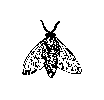
\includegraphics{fly}
% \caption{A sample black and white graphic.}
% \end{figure}

% \begin{figure}
% 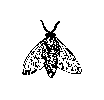
\includegraphics[height=1in, width=1in]{fly}
% \caption{A sample black and white graphic
% that has been resized with the \texttt{includegraphics} command.}
% \end{figure}


% As was the case with tables, you may want a figure that spans two
% columns.  To do this, and still to ensure proper ``floating''
% placement of tables, use the environment \textbf{figure*} to enclose
% the figure and its caption.  And don't forget to end the environment
% with \textbf{figure*}, not \textbf{figure}!

% \begin{figure*}
% 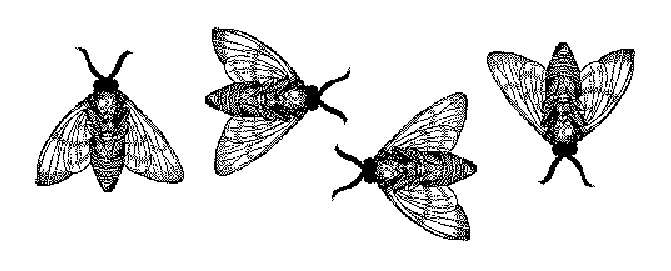
\includegraphics{flies}
% \caption{A sample black and white graphic
% that needs to span two columns of text.}
% \end{figure*}


% \begin{figure}
% 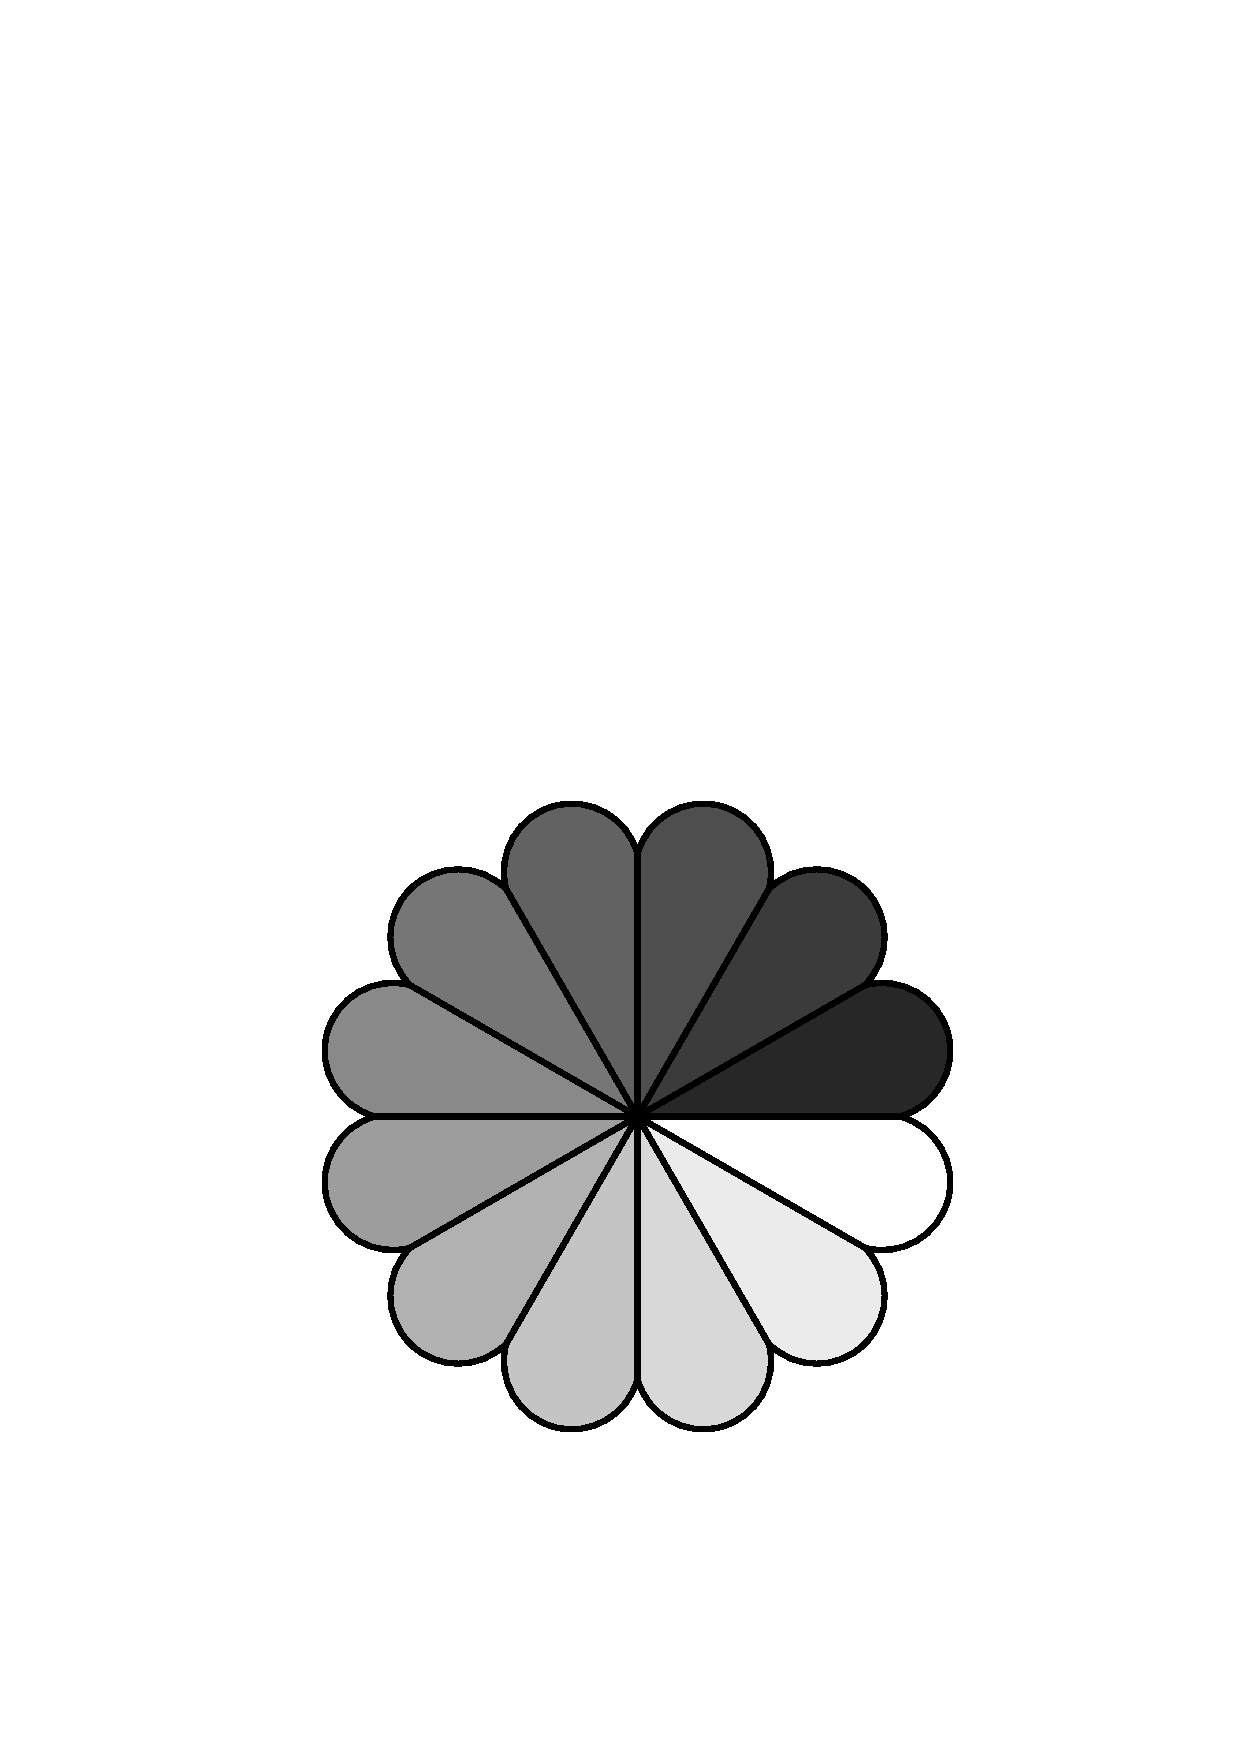
\includegraphics[height=1in, width=1in]{rosette}
% \caption{A sample black and white graphic that has
% been resized with the \texttt{includegraphics} command.}
% \end{figure}

% \subsection{Theorem-like Constructs}

% Other common constructs that may occur in your article are the forms
% for logical constructs like theorems, axioms, corollaries and proofs.
% ACM uses two types of these constructs:  theorem-like and
% definition-like.

% Here is a theorem:
% \begin{theorem}
%   Let $f$ be continuous on $[a,b]$.  If $G$ is
%   an antiderivative for $f$ on $[a,b]$, then
%   \begin{displaymath}
%     \int^b_af(t)\,dt = G(b) - G(a).
%   \end{displaymath}
% \end{theorem}

% Here is a definition:
% \begin{definition}
%   If $z$ is irrational, then by $e^z$ we mean the
%   unique number that has
%   logarithm $z$:
%   \begin{displaymath}
%     \log e^z = z.
%   \end{displaymath}
% \end{definition}

% The pre-defined theorem-like constructs are \textbf{theorem},
% \textbf{conjecture}, \textbf{proposition}, \textbf{lemma} and
% \textbf{corollary}.  The pre-defined de\-fi\-ni\-ti\-on-like constructs are
% \textbf{example} and \textbf{definition}.  You can add your own
% constructs using the \textsl{amsthm} interface~\cite{Amsthm15}.  The
% styles used in the \verb|\theoremstyle| command are \textbf{acmplain}
% and \textbf{acmdefinition}.

% Another construct is \textbf{proof}, for example,

% \begin{proof}
%   Suppose on the contrary there exists a real number $L$ such that
%   \begin{displaymath}
%     \lim_{x\rightarrow\infty} \frac{f(x)}{g(x)} = L.
%   \end{displaymath}
%   Then
%   \begin{displaymath}
%     l=\lim_{x\rightarrow c} f(x)
%     = \lim_{x\rightarrow c}
%     \left[ g{x} \cdot \frac{f(x)}{g(x)} \right ]
%     = \lim_{x\rightarrow c} g(x) \cdot \lim_{x\rightarrow c}
%     \frac{f(x)}{g(x)} = 0\cdot L = 0,
%   \end{displaymath}
%   which contradicts our assumption that $l\neq 0$.
% \end{proof}

% \section{Conclusions}
% This paragraph will end the body of this sample document.
% Remember that you might still have Acknowledgments or
% Appendices; brief samples of these
% follow.  There is still the Bibliography to deal with; and
% we will make a disclaimer about that here: with the exception
% of the reference to the \LaTeX\ book, the citations in
% this paper are to articles which have nothing to
% do with the present subject and are used as
% examples only.
% %\end{document}  % This is where a 'short' article might terminate



% \appendix
% %Appendix A
% \section{Headings in Appendices}
% The rules about hierarchical headings discussed above for
% the body of the article are different in the appendices.
% In the \textbf{appendix} environment, the command
% \textbf{section} is used to
% indicate the start of each Appendix, with alphabetic order
% designation (i.e., the first is A, the second B, etc.) and
% a title (if you include one).  So, if you need
% hierarchical structure
% \textit{within} an Appendix, start with \textbf{subsection} as the
% highest level. Here is an outline of the body of this
% document in Appendix-appropriate form:
% \subsection{Introduction}
% \subsection{The Body of the Paper}
% \subsubsection{Type Changes and  Special Characters}
% \subsubsection{Math Equations}
% \paragraph{Inline (In-text) Equations}
% \paragraph{Display Equations}
% \subsubsection{Citations}
% \subsubsection{Tables}
% \subsubsection{Figures}
% \subsubsection{Theorem-like Constructs}
% \subsubsection*{A Caveat for the \TeX\ Expert}
% \subsection{Conclusions}
% \subsection{References}
% Generated by bibtex from your \texttt{.bib} file.  Run latex,
% then bibtex, then latex twice (to resolve references)
% to create the \texttt{.bbl} file.  Insert that \texttt{.bbl}
% file into the \texttt{.tex} source file and comment out
% the command \texttt{{\char'134}thebibliography}.
% % This next section command marks the start of
% % Appendix B, and does not continue the present hierarchy
% \section{More Help for the Hardy}

% Of course, reading the source code is always useful.  The file
% \path{acmart.pdf} contains both the user guide and the commented
% code.

% \begin{acks}
%   The authors would like to thank Dr. Yuhua Li for providing the
%   MATLAB code of the \textit{BEPS} method.

%   The authors would also like to thank the anonymous referees for
%   their valuable comments and helpful suggestions. The work is
%   supported by the \grantsponsor{GS501100001809}{National Natural
%     Science Foundation of
%     China}{http://dx.doi.org/10.13039/501100001809} under Grant
%   No.:~\grantnum{GS501100001809}{61273304}
%   and~\grantnum[http://www.nnsf.cn/youngscientists]{GS501100001809}{Young
%     Scientists' Support Program}.

% \end{acks}


\bibliographystyle{ACM-Reference-Format}
\bibliography{sample-bibliography} 

\end{document}
